% !TeX spellcheck = en_US
\section{How is the decline of HPV affected if the average number of LSPs increases significantly?}

The data used to build the network model and to perform the calibration have more than $10$ years. Also, the sexual behavior of the people has changed in the last years and therefore, it would be interesting to perform some simulations adapting the model parameters to the new sexual behavior and also, we perform a sensitivity analysis of the model. Here, we propose an increasing in the number of lifetime sexual partners (LSP) of the nodes.

The simulation is going to be a little bit tricky. 

\begin{enumerate}
	\item The assignment of heterosexual LSPs follows the data in Tables \ref{tableLSPValues_men} and \ref{tableLSPValues_women}. We are going to maintain the percentages but changing the number of LSPs. Thus, the proportion of people with only 1 LSP, in the simulation will have 2; people with 2 LSPs will have 4; people with $3-4$ LSPs will have $6-8$; people with $5-9$ LSPs will have $9-13$ and the people with 10 or more LSPs will have 14 or more.
	\item The parameter determining the average number of LSPs in men will be increased in 8. Then, the values of the average number of LSPs in men corresponding to the $30$ selected simulations during the calibration (\ref{laselegidas}) will increase in 8, in order to guarantee that there are enough sexual partners available to create all the couples.
	\item In \cite{Durex2002}, we have the number of LSPs in MSM: 18 LSPs for the age group 14-19; 25 LSPs for the age group 20-24; 33 LSPs for the age group 25-29; 45 LSPs for the age group 30-39; 59 LSPs for the age group 40-49; 50 LSPs for the age group 50-59; 56 LSPs for the age group 60-85+. There number of LSPs will be increased by 4.   
\end{enumerate}

Grosso modo, in this simulation, we are increasing the LSPs in more than $100\%$. We assume the Spanish scenario where only girls are vaccinated with a $70\%$ coverage. In Figure \ref{fig:compara_k} we can see graphically the obtained results. 

\begin{figure}[!]
	\centering
	\begin{tabular}{cc}
		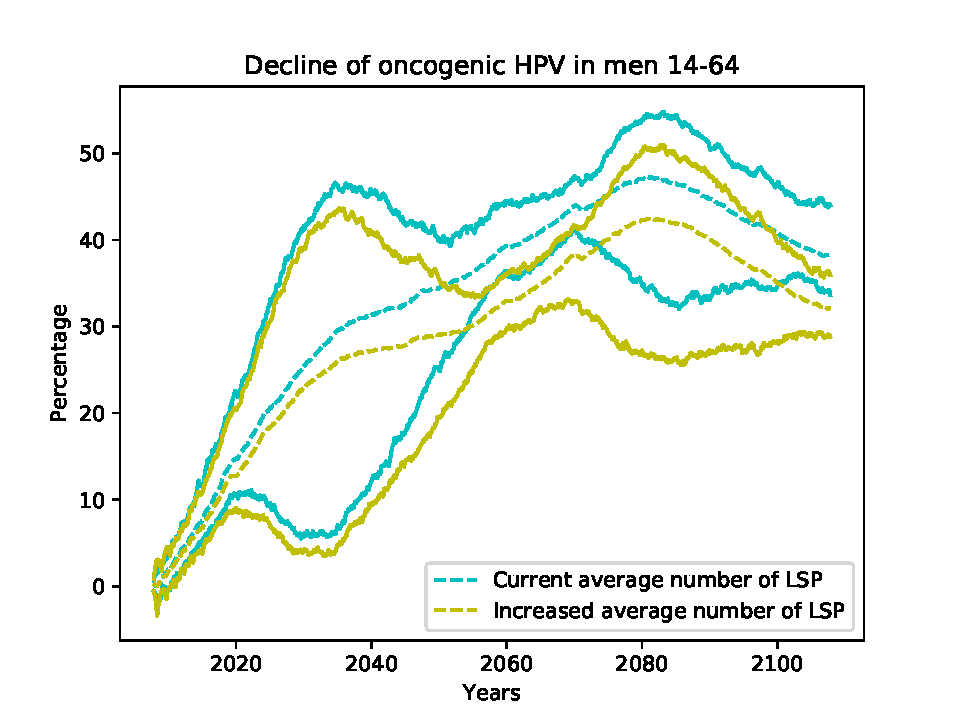
\includegraphics[width=0.5\linewidth]{IMGs/12.-Aumento_LSP/onco_hom.pdf}	& 
		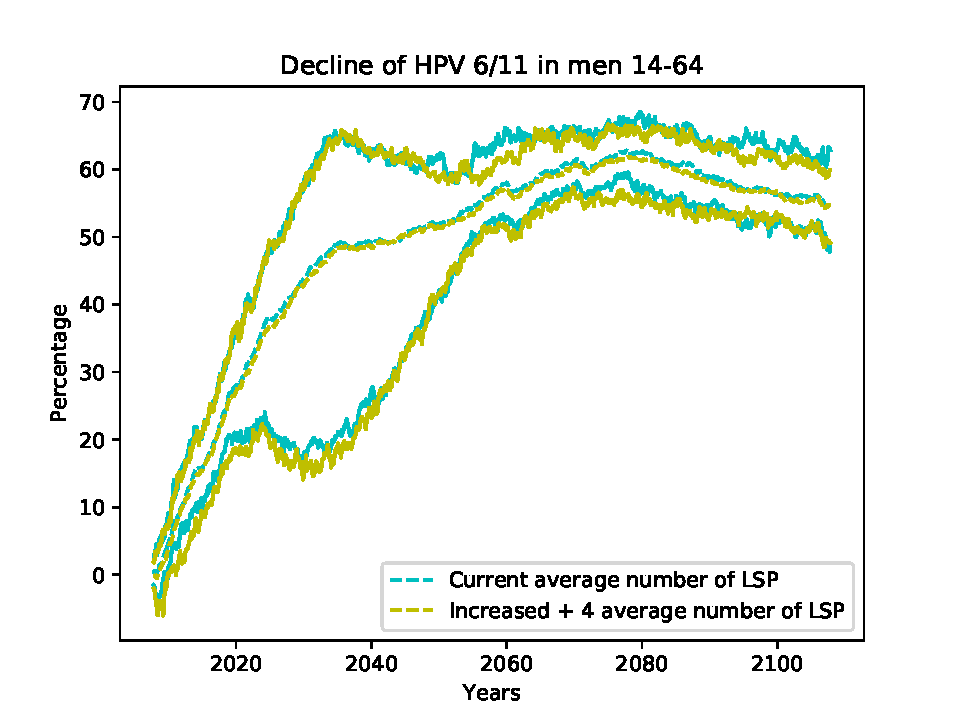
\includegraphics[width=0.5\linewidth]{IMGs/12.-Aumento_LSP/verr_hom.pdf}  \\ 
		Decline oncogenic HPV men	& Decline HPV 6/11 men \\ 
		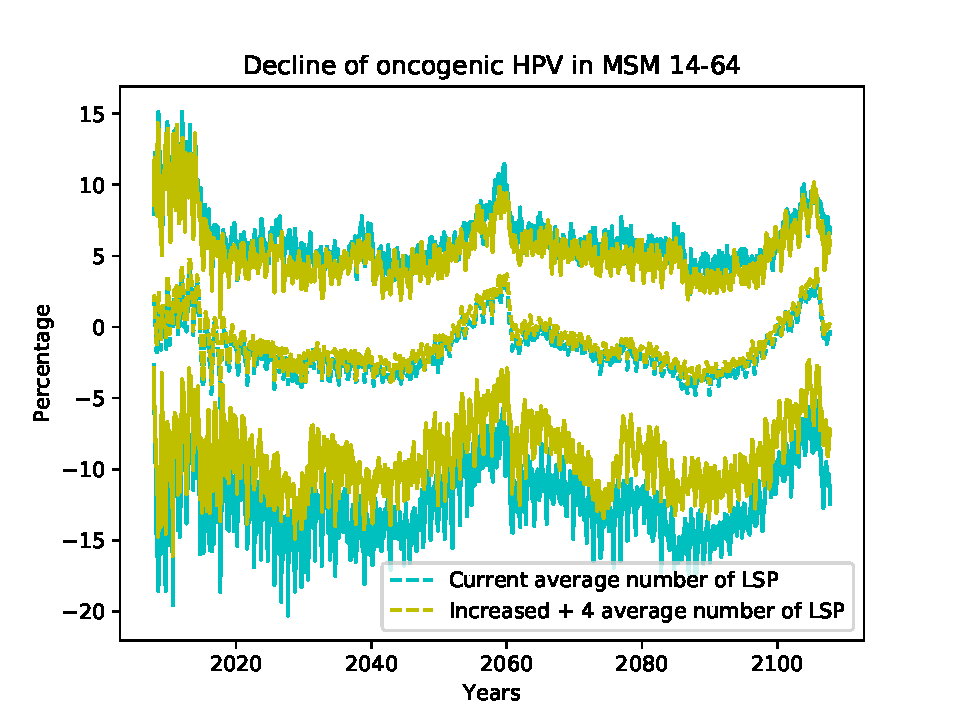
\includegraphics[width=0.5\linewidth]{IMGs/12.-Aumento_LSP/onco_MSM.pdf}	& 
		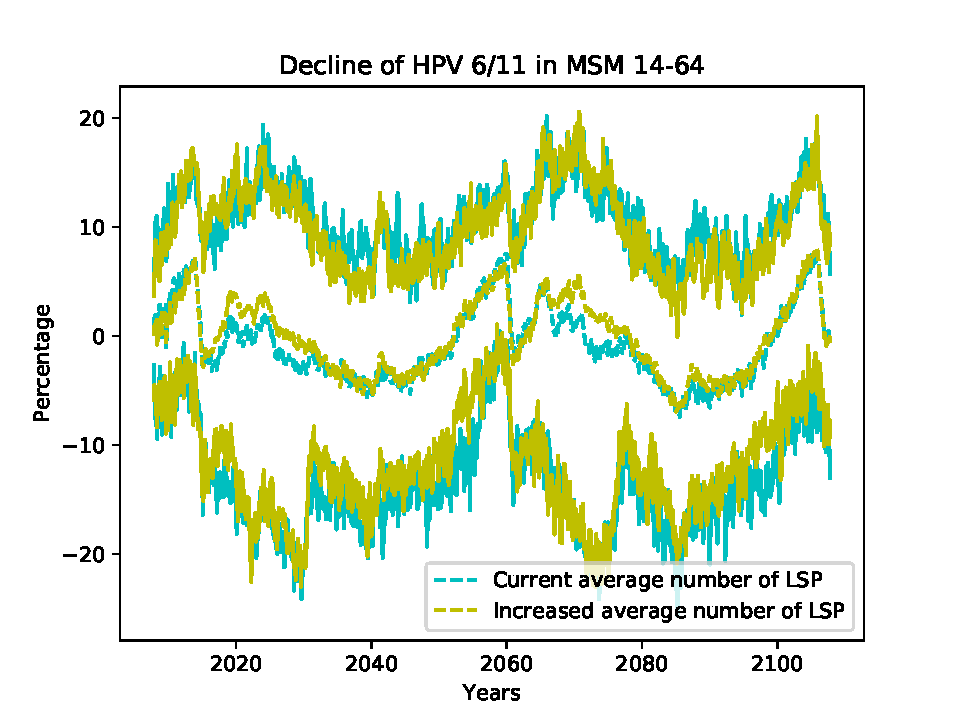
\includegraphics[width=0.5\linewidth]{IMGs/12.-Aumento_LSP/verr_MSM.pdf}  \\ 
		Decline oncogenic HPV MSM	& Decline HPV 6/11 MSM \\ 
		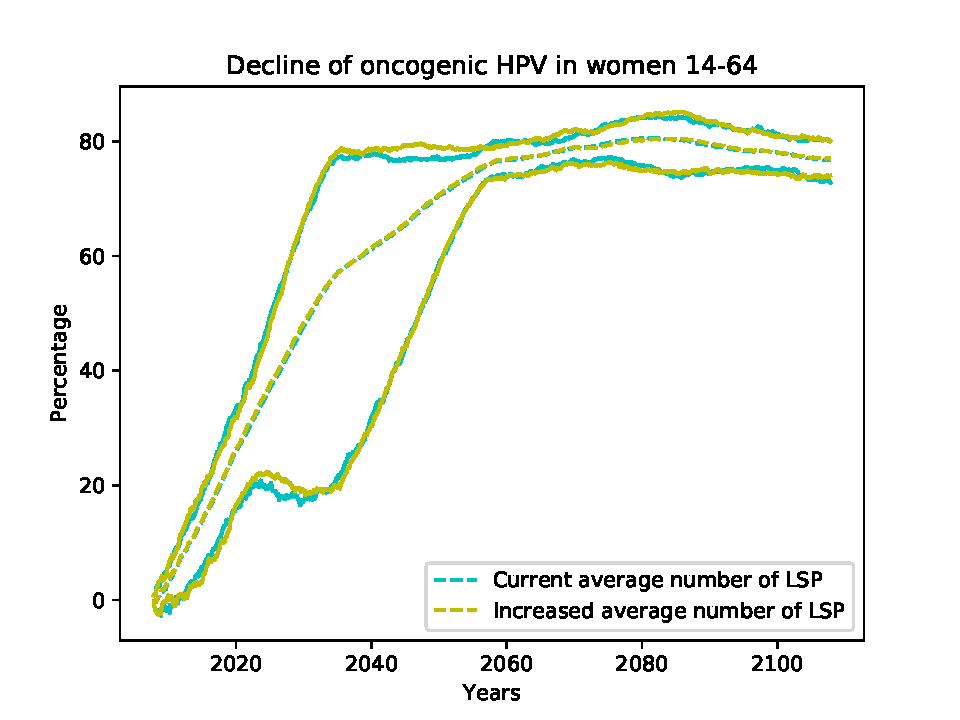
\includegraphics[width=0.5\linewidth]{IMGs/12.-Aumento_LSP/onco_muj.pdf}	& 
		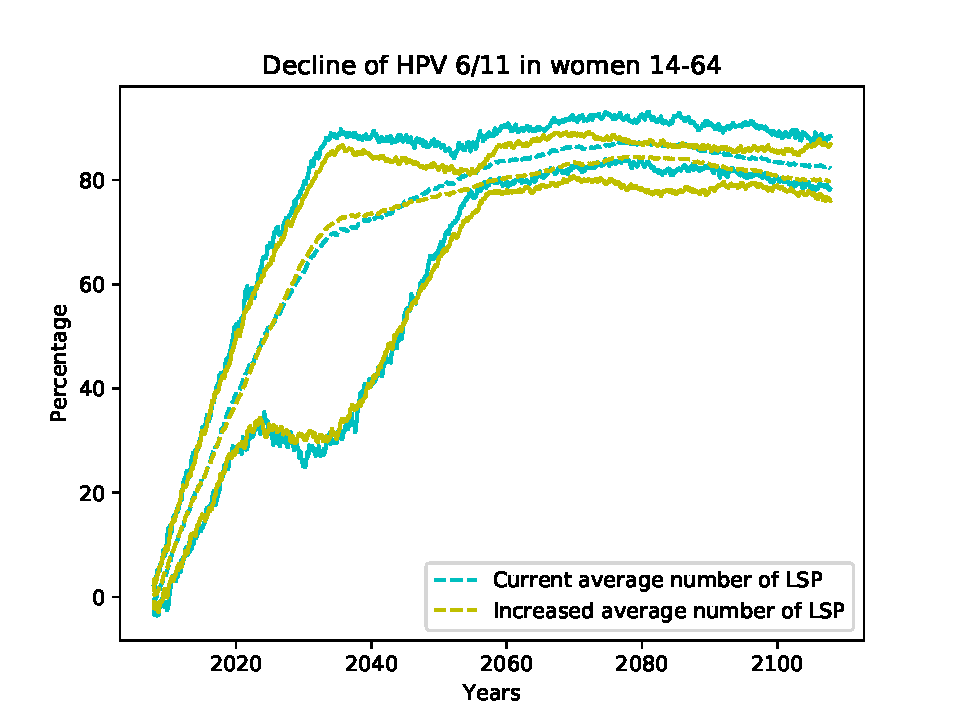
\includegraphics[width=0.5\linewidth]{IMGs/12.-Aumento_LSP/verr_muj.pdf}  \\ 
		Decline oncogenic HPV women	& Decline HPV 6/11 women \\ 
	\end{tabular} 
	\caption{Comparative of the decline of HPV in case the global average number of LSP increases. In the current vaccination scenario (vaccinating only girls with a coverage of $70\%$, there are only significant changes in declines for oncogenic HPV in men.}
	\label{fig:compara_k}
\end{figure}

The simulated increase in the number of LSPs provide small changes in the decline of the HPV infections in the long-run. The differences are between

\begin{itemize}
	\item $4.3\% - 6.4\%$ for oncogenic HPV in men,
	\item $0\% - 2.6\%$ for HPV 6/11 in men,
	\item $3.3\% - 4.5\%$ for oncogenic HPV in women,
	\item $2.0\% - 3.7\%$ for HPV 6/11 in women.	
\end{itemize}

Despite the noticeable increase in the number of LSPs, there is only a small effect on the decline of the HPV infections. Therefore, although the sexual behavior has changed in the last years and the number of sexual partners has increased, the herd immunity effect remains stable and it is not expected perceptible changes in the decline of the infection.

However, it may change if the increase in LSPs is much higher. In the Figure 2 of paper \cite{acedo2011using}, the authors study the average number of contacts for the transmission dynamics of the Respiratory Syncytial Virus (RSV). They found that the average number of contacts should take values greater than 25 to explain the dynamics of the disease.

The network defined in \cite{acedo2011using} has the same structure as the MSM LSP network, with average number of contacts (LSPs) of $39$ \cite{Durex2002}. In infectious diseases as smallpox, varicella, influenza, RSV, etc., where there are not restrictions in the possible contagious contacts, the classical and network epidemiological models say that the herd immunity effect only appears when the vaccination coverage achieves high percentages. This fact explain what we have seen along this dissertation: MSM do not have herd immunity effect when only girls are vaccinated and some herd immunity is achieved if boys, and therefore MSM, are also vaccinated with high rates of coverage.

On the other hand, with the obvious caveat that the structure of the heterosexual LSP network is not the same as the one in the random network in \cite{acedo2011using}, a strong increase in the number of average LSPs to values close to the average number of LSPs of MSM, $39$, or greater, it is possible that the herd immunity effect provided by the vaccine may be reduced significantly or disappears in the heterosexual network. As a consequence,  HPV would become a disease with a transmission dynamics similar to smallpox, varicella or influenza. 
